\section{Força magnética}

\frame{
	\frametitle{Força magnética}
	\begin{block}{Introdução}
		Anteriormente estudamos o campo magnético gerado por um fio, por uma bobina, e por um solenoide. Além disso vimos como é calculado a intensidade do vetor campo magnético $\vec{B}$.
		\begin{itemize}
			\item Agora será abordado o tema \textbf{força magnética}. Quando uma carga ou um fio percorrido por corrente são inseridos em um campo magnético, dizemos que eles sofrem a ação de uma força magnética.
		\end{itemize}
	\end{block}
}

\frame{
	\frametitle{Força magnética}
	\begin{block}{Definição}
		A força magnética, ou \textbf{força de Lorentz}, é resultado da interação entre dois corpos dotados de \textbf{propriedades magnéticas}, como ímãs ou cargas elétricas em movimento.
	\end{block}
}

\frame{
	\frametitle{Força magnética}
	\begin{block}{Contextualização}
		As auroras que circundam o polo magnético norte (boreal) e o polo magnético sul (austral) ocorrem quando elétrons de carga elevada provenientes do vento solar interagem com elementos da atmosfera terrestre. Os ventos solares fluem escapando do Sol com velocidades de cerca de 1,6 milhões de quilômetros por hora. Quando alcançam a Terra cerca de 40 horas depois de deixarem o Sol, seguem linhas de força magnética geradas pelo núcleo da Terra, fluindo através da magnetosfera por uma área com formato de lágrima constituída de campos magnéticos e elétricos de alta carga.
	\end{block}
	\centerline{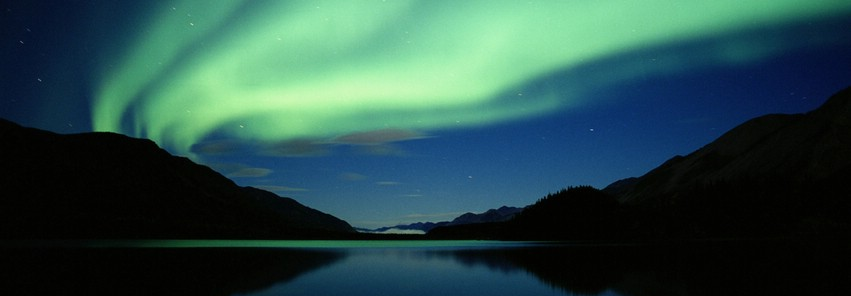
\includegraphics[width=0.6\linewidth]{Figuras/Ch09/fig1.png}}
}

\frame{
	\frametitle{Força magnética sobre uma carga elétrica}
	\begin{block}{Definição}
		Para corpos de dimensões desprezíveis, a força magnética $\vec{F_m}$ sobre partículas carregadas tem as seguintes características:
		\begin{itemize}
			\item \textbf{Direção}: perpendicular aos vetores velocidade e campo magnético.
			\item \textbf{Sentido}: obtido através da regra da mão esquerda.
			\item \textbf{Intensidade}:
			      $$\boxed{|\vec{F_m}| = q \cdot |\vec{v}| \cdot |\vec{B}| \sen \theta}$$
		\end{itemize}
	\end{block}
}

\frame{
	\frametitle{Força magnética sobre uma carga elétrica}
	\begin{block}{Unidades}
		$$|\vec{F_m}| = q \cdot \vec{v} \cdot \vec{B} \sen \theta$$
		\begin{itemize}
			\item $|\vec{F_m}|$: força magnética, em \si{\newton}.
			\item $q$: carga elétrica líquida, em \si{\coulomb}.
			\item $|\vec{v}|$: velocidade da partícula em relação a $\vec{B}$, em \textbf{\si{\meter\per\second}}.
			\item $|\vec{B}|$: vetor campo magnético, em \si{\tesla}.
			\item $\theta$: ângulo formado entre $\vec{B}$ e $\vec{v}$, em graus.
		\end{itemize}
	\end{block}
}

\frame{
	\frametitle{Força magnética sobre uma carga elétrica}
	\begin{block}{Regra da mão esquerda}
		A regra da mão esquerda, chamada de ``regra da mão esquerda de Fleming'', é usada para encontrar o \textbf{sentido da força magnética}.
		\begin{itemize}
			\item O dedo \textbf{polegar} representa o sentido da força magnética ($\vec{F_m}$).
			\item Já o dedo \textbf{indicador} representa o campo magnético ($\vec{B}$).
			\item O dedo \textbf{médio} indica o sentido da velocidade ($\vec{v}$).
		\end{itemize}
	\end{block}
	\centerline{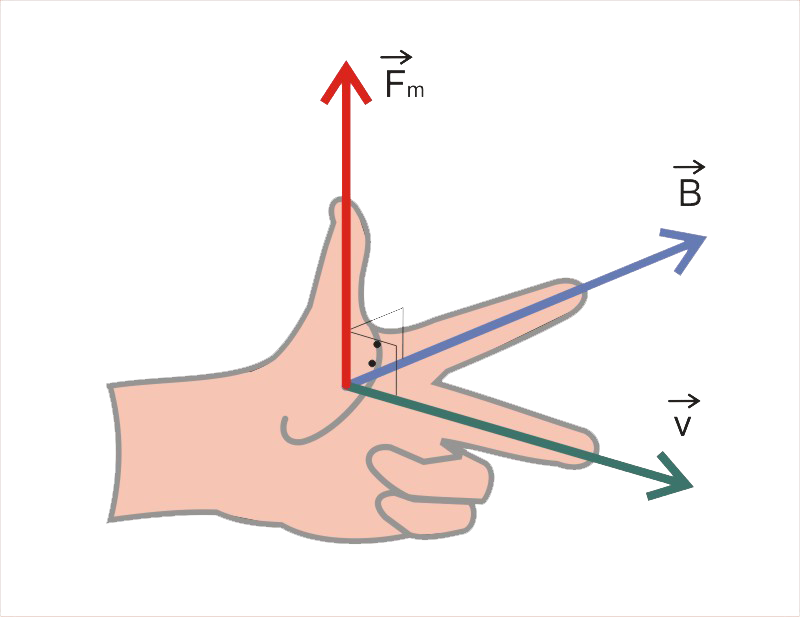
\includegraphics[width=0.45\linewidth]{Figuras/Ch09/fig2.png}}
}

\frame{
	\frametitle{Força magnética sobre uma carga elétrica}
	\begin{block}{Exemplo}
		Na figura abaixo, temos duas partículas carregadas (em vermelho) deslocando-se com velocidade $\vec{v}$ em uma região onde o campo magnético é constante e vertical para cima. O sentido da força magnética depende da regra da mão esquerda.
	\end{block}

	\centering
	\setmyunit{1cm}
	\begin{tikzpicture}
		\draw (1,2.5) rectangle +(0.1,0.1) node[pos=.5] {$ \cdot $};
	
		\foreach \x in {0,1,2,3}{
			\draw[blue,-Latex] (\x,0) -- (\x,3); 
		}
	
		\draw[blue] (2.8,3) node {$ \vec{B} $};
	
		\fill[red] (0.6,2.5) circle (1ex);
		\draw[-Latex,red] (0.6,2.5) -- node[below,xshift=3pt] {$ \vec{v} $} (1.6,2.5);
	
		\draw (0.6,1.5) circle (1ex) node[below left=0.8ex] {$ \vec{F} $};
		\fill (0.6,1.5) circle (0.75ex);
	
		\draw (2.5,1) circle (1ex) node[below left=0.8ex] {$ \vec{F} $} (2.5,1) -- ++(0.375ex,0.375ex) -- ++(-0.75ex,-0.75ex) ++(0,0.75ex) -- ++(0.75ex,-0.75ex);
		
		\fill[red] (3.3, 1.2) circle (1ex);
		\draw[red,-Latex] (3.3,1.2) -- node[below] {$ \vec{v} $} +(-30:-1);
		
		
		\path[name path=arb] (3,0) -- (3,3);
		\path[name path=arv] (3.3,1.2) -- +(-30:-1);
		
		\coordinate (A) at (3,3);
		\draw[name intersections={of=arb and arv, by=x}] (x) node[coordinate,name=O] {};
		\coordinate (B) at ($ (3.3,1.2)+(-30:-1) $);
		
		\pic[draw, angle radius=10pt,angle eccentricity=1,"$ \theta $" {xshift=-4pt,yshift=4pt}] {angle=A--O--B};
	\end{tikzpicture}	
%	\centerline{
\includegraphics[width=0.35\linewidth]{Figuras/Ch09/fig3.jpg}}
}

\frame{
	\frametitle{Força magnética sobre uma carga elétrica}
	\begin{block}{Atenção}
		O sentido da força magnética dado pela regra da mão esquerda é para uma carga $q$ \textbf{positiva}.
		\begin{itemize}
			\item Se a carga da partícula for \textbf{negativa}, basta \textbf{inverter o sentido do dedão}. Utilize a regra da mesma forma e, no final, inverta: se o dedão aponta para cima, a força magnética aponta para baixo e vice-versa.
		\end{itemize}
	\end{block}
}

\frame{
	\frametitle{Força magnética sobre uma carga elétrica}
	\begin{block}{Movimento de uma partícula eletrizada num campo magnético uniforme}
		Considere uma partícula eletrizada com carga elétrica $q$, lançada com velocidade $\vec{v}$ num campo magnético uniforme de indução $\vec{B}$. Dependendo do ângulo $\theta$ formado entre $\vec{v}$ e $\vec{B}$ a partícula pode descrever um dos movimentos:
		\begin{enumerate}
			\item \textbf{MRU} (movimento retilíneo uniforme).
			\item \textbf{MCU} (movimento circular uniforme).
			\item \textbf{MHU} (movimento helicoidal uniforme).
		\end{enumerate}
	\end{block}
}

\frame{
	\frametitle{Força magnética sobre uma carga elétrica}
	\begin{block}{\textbf{MRU} (movimento retilíneo uniforme)}
		\textbf{Quando a partícula lançada possui velocidade paralela às linhas de indução do campo magnético, a força magnética é nula}.
		\begin{itemize}
			\item Observe que, nesse caso, o ângulo $\theta = \ang{0}$ ou $\theta = \ang{180}$, e portanto
			      $$|\vec{F_m}| = q \cdot |\vec{v}| \cdot |\vec{B}| \cdot \sen \theta = q \cdot |\vec{v}| \cdot |\vec{B}| \cdot 0 = 0$$
			\item Se a força é igual a zero, a partícula mantém-se com a \textbf{mesma velocidade e realiza movimento retilíneo uniforme na mesma direção do campo magnético}.
		\end{itemize}
	\end{block}

	\setmyunit{1cm}

	\begin{minipage}{0.49\linewidth}
		\centering
		\begin{tikzpicture}
			\foreach \x in {1,2,3} {
				\draw[blue,-Latex] (0,\x) -- (3,\x); 
			}
			\draw[blue] (2.8,2.5) node {$ \vec{B} $};
		
			\fill (0.5,1.5) circle (1ex) node[left=0.8ex] {$ q $};
			\draw[-Latex] (0.5,1.5) -- (1.5,1.5) node[right] {$ \vec{v} $};
			
		\end{tikzpicture}
	\end{minipage}
	\hfill
	\begin{minipage}{0.49\linewidth}
		\centering
		\begin{tikzpicture}
		\foreach \x in {1,2,3} {
			\draw[blue,-Latex] (0,\x) -- (3,\x); 
		}
		\draw[blue] (2.8,2.5) node {$ \vec{B} $};
		
		\fill (1.5,1.5) circle (1ex) node[right=0.8ex] {$ q $};
		\draw[-Latex] (1.5,1.5) -- (0.5,1.5) node[left] {$ \vec{v} $};
		
		\end{tikzpicture}
	\end{minipage}

%	\centerline{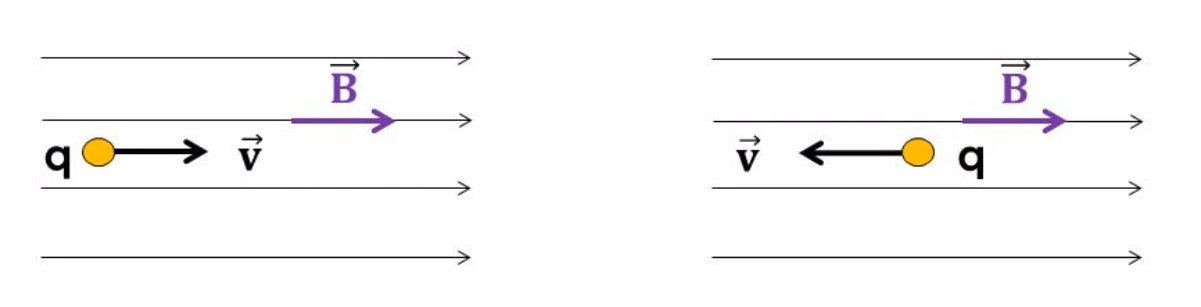
\includegraphics[width=0.9\linewidth]{Figuras/Ch09/fig4.PNG}}
}

\frame{
	\frametitle{Força magnética sobre uma carga elétrica}
	\begin{block}{\textbf{MCU} (movimento circular uniforme)}
		\textbf{Quando a partícula lançada possui velocidade perpendicular às linhas de indução do campo magnético, a força magnética é máxima}.
		\begin{itemize}
			\item Observe que, nesse caso, o ângulo $\theta = \ang{90}$, e portanto
			      $$|\vec{F_m}| = q \cdot |\vec{v}| \cdot |\vec{B}| \cdot \sen \theta = q \cdot |\vec{v}| \cdot |\vec{B}| \cdot 1 = q \cdot |\vec{v}| \cdot |\vec{B}|$$
		\end{itemize}
	\end{block}

	\centering
	\setmyunit{0.5cm}
	
	\begin{tikzpicture}
		\pgfmathsetmacro{\len}{0.2}
		\pgfmathsetmacro{\hlen}{\len/2}
	
		\foreach \i in {-3,-2,...,3} {
			\foreach \j in {-3,-2,...,3} {
				\draw[blue] (\i,\j) -- ++(\hlen,\hlen) -- ++(-\len,-\len) ++(0,\len) -- ++(\len,-\len);
			}
		}
	
		\draw[blue] (3.5,2.5) node[] {$ \vec{B} $};
		
		\draw[dashed,thick] (0,0) circle (2.5);
		
		\coordinate (q) at ($ (0,0)+(-30:2.5) $);
		
		\draw[-Latex] (q) -- node[above] {$ \vec{F} $} ($ (q)!0.6!(0,0) $);
		\draw[-Latex,red] (q) -- node[right] {$ \vec{v} $} +(60:2);
		\filldraw[fill=white,draw=black] (q) circle (1ex) node[fill=white,inner sep=1pt,below left=1ex] {$ q $};
		\node at (q) {\footnotesize $ + $};
	\end{tikzpicture}
	
%	\centerline{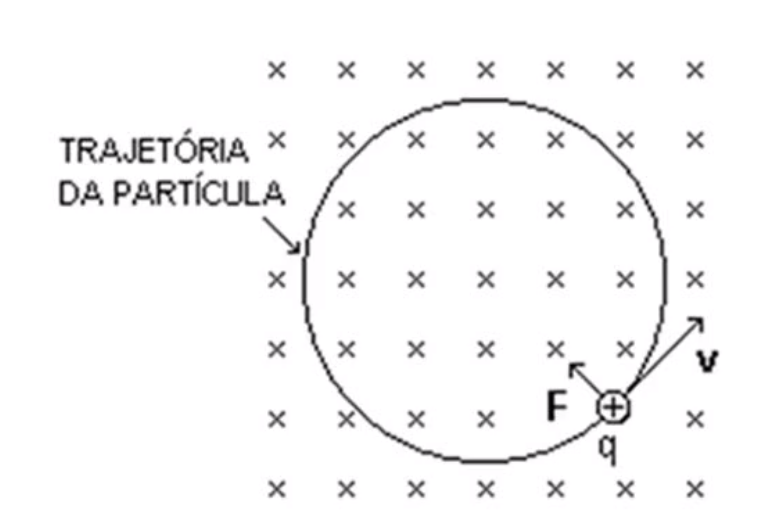
\includegraphics[width=0.5\linewidth]{Figuras/Ch09/fig5.PNG}}
}

\frame{
	\frametitle{Força magnética sobre uma carga elétrica}
	\begin{block}{\textbf{MCU} (movimento circular uniforme)}
		\begin{itemize}
			\item O movimento executado pela partícula é circular e uniforme, e o raio de sua trajetória é obtido da seguinte forma:
			      $$|\vec{F_m}| = |\vec{F_{cp}}| \implies q \cdot |\vec{v}| \cdot |\vec{B}| = \dfrac{m \cdot |\vec{v}|^2}{R} \implies \boxed{R = \dfrac{m \cdot |\vec{v}|}{q \cdot |\vec{B}|}}$$
			\item Para calcular o período ($T$), que é o intervalo de tempo que a partícula leva para completar uma volta, utilizamos:
			      $$S = S_0 + \vec{v} \cdot T \implies \Delta S = \vec{v} \cdot t \implies 2\pi \cdot R = \vec{v} \cdot T \implies 2\pi \cdot \dfrac{m \cdot |\vec{v}|}{q \cdot |\vec{B}|} = \vec{v} \cdot T$$ $$\boxed{T = \dfrac{2\pi \cdot m}{q \cdot |\vec{B}|}}$$
		\end{itemize}
	\end{block}
}

\frame{
	\frametitle{Força magnética sobre uma carga elétrica}
	\begin{block}{\textbf{MHU} (movimento helicoidal uniforme)}
		\textbf{Quando a partícula lançada possui velocidade oblíqua às linhas de indução do campo magnético, devemos considerar as componentes $\bm{x}$ e $\bm{y}$ do vetor velocidade}.
		\begin{itemize}
			\item Observe que, nesse caso, o ângulo $\theta$ é diferente de $\ang{0}$, $\ang{90}$ e $\ang{180}$.
			\item A velocidade $\vec{V_x}$ tem o mesmo sentido que as linhas de campo magnético (\textbf{MRU}), enquanto $\vec{V_y}$ é perpendicular (\textbf{MCU}). A resultante da velocidade ocasiona um movimento circular e uniforme, com direção perpendicular ao vetor $\vec{B}$, que pode ser denominado de \textbf{helicoidal uniforme}.
		\end{itemize}
	\end{block}

	\setmyunit{1cm}
	
	\begin{minipage}{0.49\linewidth}
		\centering
		\begin{tikzpicture}
		\foreach \x in {1,2,3} {
			\draw[blue,-Latex] (0,\x) -- (3,\x); 
		}
		\draw[blue] (2.8,2.5) node {$ \vec{B} $};
		
		\fill (0.5,1.5) circle (1ex) node[left=0.8ex] {$ q $};
		\draw[-Latex] (0.5,1.5) -- +(1,1) node[right] {$ \vec{v} $};
		
		\end{tikzpicture}
	\end{minipage}
	\hfill
	\begin{minipage}{0.49\linewidth}
		\centering
		\begin{tikzpicture}[ar/.style={dashed,postaction={decorate,decoration={
					post length=1mm,
					pre length=1mm,markings,mark=between positions 0.05 and 0.95 step 0.4 with {\arrow{Latex}}
		}}}]
		\foreach \x in {1,2,3} {
			\draw[blue,-Latex] (0,\x) -- (3,\x); 
		}
		\draw[blue] (2.8,2.7) node {$ \vec{B} $};
		
		% 0.3 ... how far the rings are apart
		% 0.4 ... how much from the side the rings are seen (try 0 and the same as the radius)
		% 1.5 ... radius of the rings
		\def\coil####1{
			{0.3 * (2*####1 + \t) + -0.3*sin(\t * pi r))-0.8},
			{0.8 * cos(\t * pi r)+2}
		}
		
		\foreach \n in {1,2,...,3} {
			\draw[ar,domain={1:3},smooth,variable=\t,samples=15]
			plot (\coil{\n}); 
		}
	
		\draw[dashed,postaction={decorate,decoration={
				post length=1mm,
				pre length=1mm,markings,mark=at position 0.25 with {\arrow{Latex}}
		}},domain={1:1.65},smooth,variable=\t,samples=4]
		plot (\coil{4});
%		
		\fill (2.35,2.45) circle (1ex) node[left=0.7ex] {$ q $};
		
		\draw[-Latex] (2.35,2.45) -- node[below] {$ \vec{v_x} $} +(1,0);
		\draw[-Latex] (2.35,2.45) -- node[left] {$ \vec{v_y} $} +(0,0.7);
		
		\end{tikzpicture}
	\end{minipage}
%	\centerline{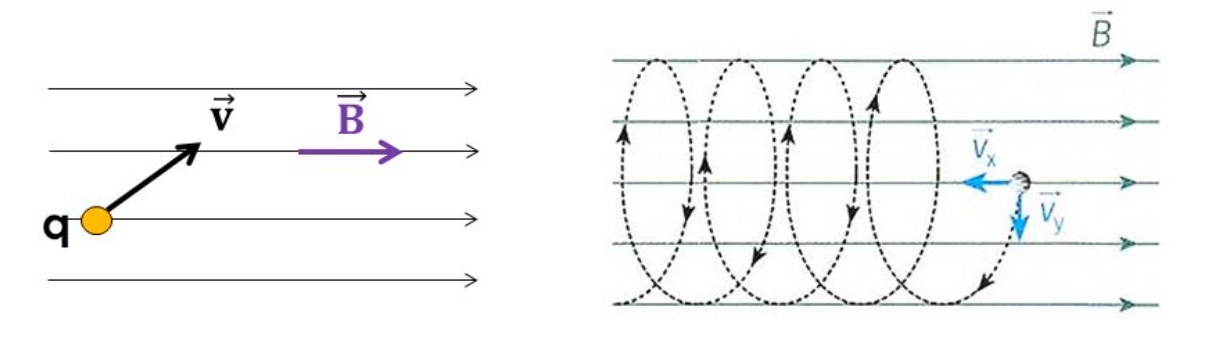
\includegraphics[width=0.9\linewidth]{Figuras/Ch09/fig6.PNG}}
}

\frame{
	\frametitle{Força magnética sobre uma carga elétrica}
	\begin{block}{\textbf{MHU} (movimento helicoidal uniforme)}
		\begin{itemize}
			\item A composição de um MRU e um MCU em planos perpendiculares resulta num movimento helicoidal uniforme. A trajetória é uma hélice cilíndrica.
			      $$\boxed{R = \dfrac{m \cdot \vec{V_y}}{q \cdot \vec{B}}}$$
			\item A distância que a partícula avança por período $t$ é chamada de \textbf{passo da hélice} ($P$).
			      $$\boxed{P = \vec{V_x} \cdot t}$$
		\end{itemize}
	\end{block}

	\setmyunit{1cm}
	\centering
	\scalebox{0.85}{
		\begin{tikzpicture}[ar/.style={dashed,postaction={decorate,decoration={
					post length=1mm,
					pre length=1mm,markings,mark=between positions 0.05 and 0.95 step 0.4 with {\arrow{Latex}}
		}}}]
		\foreach \x in {1,2,3} {
			\draw[blue,-Latex] (0,\x) -- (3,\x); 
		}
		\draw[blue] (2.8,2.7) node {$ \vec{B} $};
		
		% 0.3 ... how far the rings are apart
		% 0.4 ... how much from the side the rings are seen (try 0 and the same as the radius)
		% 1.5 ... radius of the rings
		\def\coil####1{
			{0.3 * (2*####1 + \t) + -0.3*sin(\t * pi r))-0.8},
			{0.8 * cos(\t * pi r)+2}
		}
		
		\foreach \n in {1,2,...,3} {
			\draw[ar,domain={1:3},smooth,variable=\t,samples=15]
			plot (\coil{\n}); 
		}
		
		\draw[dashed,postaction={decorate,decoration={
				post length=1mm,
				pre length=1mm,markings,mark=at position 0.25 with {\arrow{Latex}}
		}},domain={1:1.65},smooth,variable=\t,samples=4]
		plot (\coil{4});
		%		
		\fill (2.35,2.45) circle (1ex) node[left=0.7ex] {$ q $};
		
		\draw[-Latex] (2.35,2.45) -- node[below] {$ \vec{v_x} $} +(1,0);
		\draw[-Latex] (2.35,2.45) -- node[left] {$ \vec{v_y} $} +(0,0.7);
		
		\draw[red,<->] (1,3.2) -- node[above] {Passo ($ P $)} +(0.6,0);
		\draw[red,dashed] (1,3.2) -- +(0,-0.4);
		\draw[red,dashed] (1.6,3.2) -- +(0,-0.4);
		\end{tikzpicture}}
%	\centerline{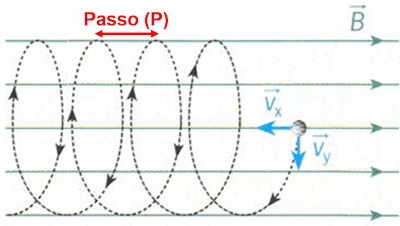
\includegraphics[width=0.4\linewidth]{Figuras/Ch09/fig7.png}}
}

\frame{
	\frametitle{Força magnética sobre uma carga elétrica - Exemplo $\#01$}
	
	\begin{block}{}
		Represente as trajetórias das partículas eletrizadas, (1) e (2). Considere que as partículas não abandonam a região na qual existe o campo magnético uniforme.
	\end{block}
	
	\vspace{0.2cm}
	
	\centering
	\setmyunit{1cm}
	\begin{tikzpicture}
		\pgfmathsetmacro{\len}{0.2}
		\pgfmathsetmacro{\hlen}{\len/2}
		
		\foreach \i in {-2.5,-1.5,...,2.5} {
			\foreach \j in {-2.5,-1.5,...,2.5} {
				\draw[blue] (\i,\j) circle (1ex);
				\fill[blue] (\i,\j) circle (0.5ex);
			}
		}
	
		\draw[blue] (3,2) node {$ \vec{B} $};
		
		\fill (-1,0.8) circle (1ex) node[left=1.2ex] {(1)} node[above=1.2ex] {$ q<0 $} (-1,-0.9) circle (1ex) node[left=1.2ex] {(2)} node[below=1.2ex] {$ q>0 $};
		
		\draw[-Latex] (-1,0.8) -- node[above] {$ \vec{v} $} +(1,0);
		\draw[-Latex] (-1,-0.9) -- node[below] {$ \vec{v} $} +(1,0);
	\end{tikzpicture}
	
%	\centerline{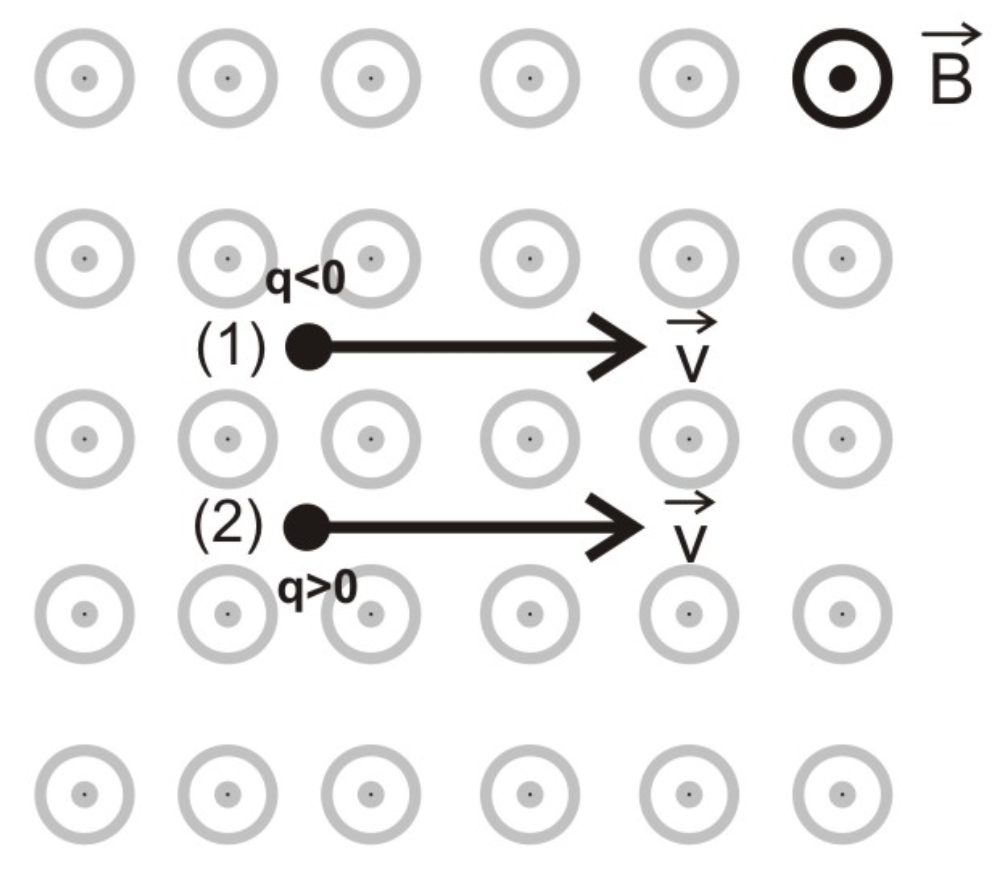
\includegraphics[width=0.4\linewidth]{Figuras/Ch09/fig8.PNG}}
}

\frame{
	\frametitle{Força magnética sobre uma carga elétrica - Exemplo $\#01$}
	\begin{block}{Resolução}
		Em cada situação determinamos, na posição de lançamento, a força magnética $\vec{F_m}$. Esta força aponta para o centro da circunferência que tangencia a velocidade $\vec{v}$.
	\end{block}
	
	\centering
	\setmyunit{0.4cm}
	
	\begin{tikzpicture}

	\draw[blue] (2.5,2) circle (1ex) node[right=1.2ex] {$ \vec{B} $};
	\fill[blue] (2.5,2) circle (0.5ex);
	
	\draw[dashed,thick,postaction={decorate,decoration={markings,mark=at position 0 with \arrow{Latex}}}] (0,0) circle (2.5);
	
	\draw (-2.5,-3) node[] {(1) $ q<0 $};
	
	\draw[-Latex] (0,-2.5) -- node[left] {$ \vec{F} $} +(0,1.5);
	\draw[-Latex,red] (0,-2.5) -- node[below] {$ \vec{v} $} +(2.5,0);
	\fill (0,-2.5) circle (1ex);
	\end{tikzpicture}
	
	\begin{tikzpicture}[yscale=-1]
	
	\path (2.5,2) circle (1ex) node[right=1.2ex,color=white] {$ \vec{B} $};
	\path (2.5,2) circle (0.5ex);
	
	\draw[dashed,thick,postaction={decorate,decoration={markings,mark=at position 0 with \arrow{Latex}}}] (0,0) circle (2.5);
	
	\draw (-2.5,-3) node[] {(2) $ q>0 $};
	
	\draw[-Latex] (0,-2.5) -- node[left] {$ \vec{F} $} +(0,1.5);
	\draw[-Latex,red] (0,-2.5) -- node[above] {$ \vec{v} $} +(2.5,0);
	\fill (0,-2.5) circle (1ex);
	\end{tikzpicture}

%	\vspace{0.2cm}
%	\centerline{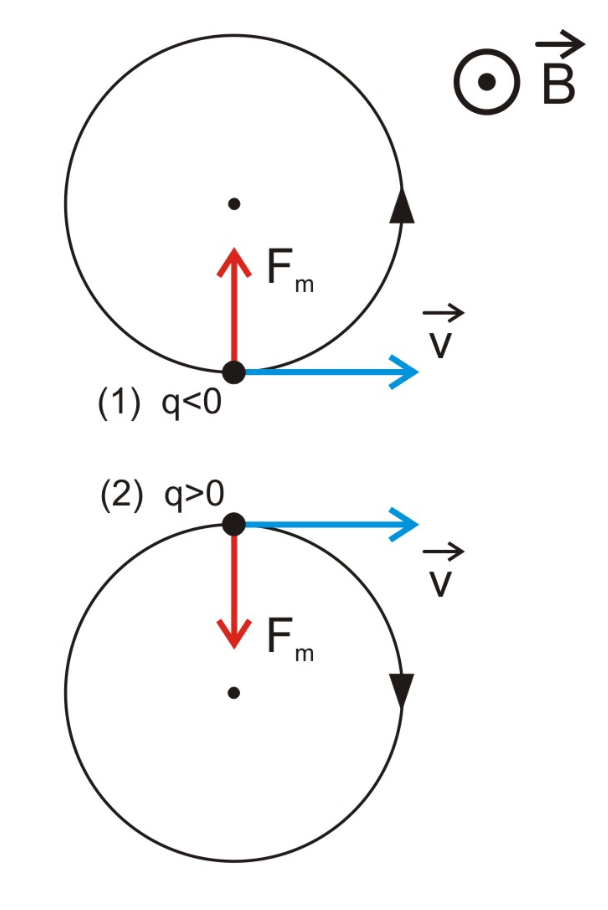
\includegraphics[width=0.3\linewidth]{Figuras/Ch09/fig9.PNG}}
}

\frame{
	\frametitle{Força magnética sobre uma carga elétrica - Exemplo $\#02$}
	\begin{block}{}
		Uma partícula de massa $m$ e eletrizada com carga elétrica $q < 0$ é lançada de um ponto $O$, com velocidade $|\vec{v}| = \SI{1e5}{\meter\per\second}$, numa região onde existe um campo magnético uniforme de intensidade $|\vec{B}| =\SI{1e-3}{\tesla}$. A partícula descreve a semi-circunferência indicada na figura, incidindo no ponto $C$ do anteparo. Sendo $q/m = \SI{1e-9}{\coulomb\per\kilo\gram}$, calcule a distância do ponto $O$ ao ponto $C$.
	\end{block}

	\medskip
	\centering
	\setmyunit{1cm}
	\begin{tikzpicture}[ground/.style={fill,pattern=north east lines,draw=none,minimum width=0.5cm,minimum height=0.3cm}]
		\draw (-3.5,0.25) -- (3.5,0.25);
		\draw[ground] (-3.5,0.25) rectangle (3.5,-0.25) node[below] {Anteparo};
		\fill[white] (-2.45,0.26) rectangle (-1.55,-0.26);
		
		\pgfmathsetmacro{\len}{0.2}
		\pgfmathsetmacro{\hlen}{\len/2}
		
		\foreach \i in {-2.5,-1.5,...,2.5} {
			\foreach \j in {1,2,3} {
				\draw[blue] (\i,\j) circle (0.2);
				\draw[blue] (\i,\j) -- ++(\hlen,\hlen) -- ++(-\len,-\len) ++(0,\len) -- ++(\len,-\len);
			}
		}
	
		\draw[blue] (3,2.5) node {$ \vec{B} $};
		
		\draw[dashed,postaction={decorate,decoration={markings,mark=between positions 0 and 1 step 0.25 with \arrow{>}}}] (-2,0.25) arc (-180:-360:2);
		
		\draw (-2,0.25) node[above left] {$ O $} (2,0.25) node[above right] {$ C $};
		
%		\fill[white] (-2,0) circle (1.5ex);
		
		\fill (-2,0.25) circle (1ex) node[below=0.2] {$ q<0 $};
		\draw[-Latex] (-2,0.25) -- node[left] {$ \vec{v} $} +(0,2);
		
	\end{tikzpicture}
	
%	\centerline{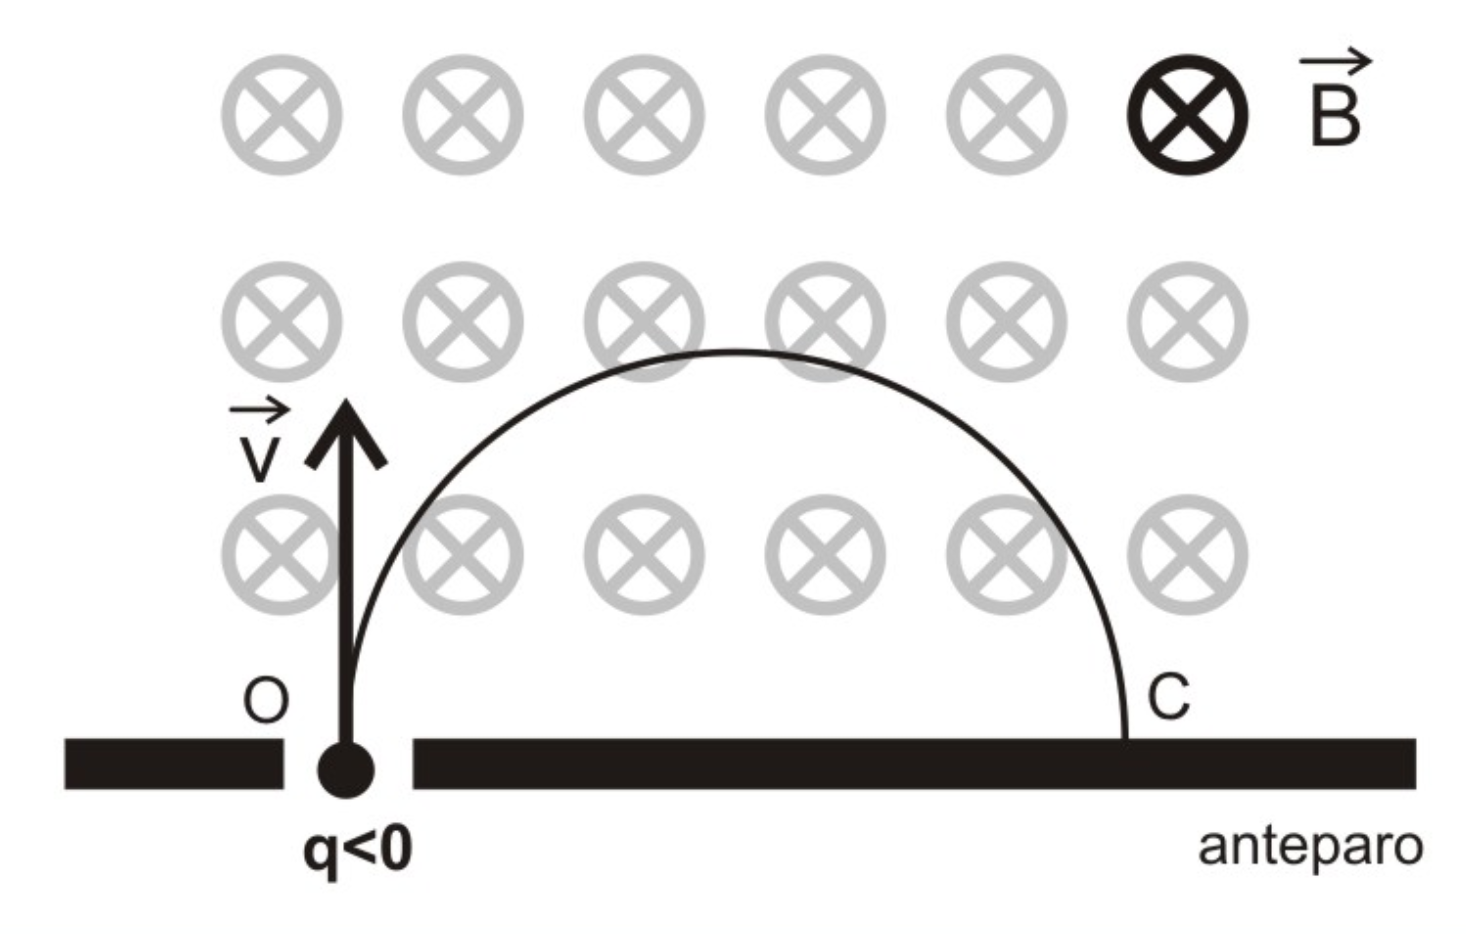
\includegraphics[width=0.5\linewidth]{Figuras/Ch09/fig10.PNG}}
}

\frame{
	\frametitle{Força magnética sobre uma carga elétrica - Exemplo $\#02$}
	\begin{block}{Resolução}
		$$R = \dfrac{m \cdot \vec{v}}{q \cdot \vec{B}} = \dfrac{\num{1e-9} \cdot \num{1e5}}{\num{1e-3}} = \SI{0.1}{\meter}$$
		Com isso, a distância do ponto $O$ ao ponto $C$ é dada por $2R = \SI{0.2}{\meter}$.
	\end{block}
}

\frame{
	\frametitle{Força magnética sobre uma carga elétrica - Exemplo $\#03$}
	\begin{block}{}
		Uma partícula de massa $m$ e carga $q$ foi lançada com velocidade $\vec{v}$ em uma região onde existem dois campos uniformes: um magnético $\vec{B}$ e outro elétrico $\vec{E}$. Verificou-se que a partícula atravessou a região com velocidade vetorial constante, em virtude de a força magnética $\vec{F_m}$ ter equilibrado a força elétrica $\vec{F_e}$, conforme a figura. (a) Qual é o sinal da carga elétrica $q$? (b) Qual é o módulo da velocidade $\vec{v}$ em função das intensidades dos campos magnético $\vec{B}$ e elétrico $\vec{E}$?
	\end{block}
	
	
	\centering
	\setmyunit{1cm}
	\begin{tikzpicture}
		\pgfmathsetmacro{\len}{0.2}
		\pgfmathsetmacro{\hlen}{\len/2}
		
		\foreach \i in {-2,-1,...,2} {
			\foreach \j in {0,1,2} {
%				\draw[blue] (\i,\j) circle (0.2);
				\draw[blue] (\i,\j) -- ++(\hlen,\hlen) -- ++(-\len,-\len) ++(0,\len) -- ++(\len,-\len);
			}
		}
	
		\fill[white] (-0.5,-0.25) rectangle (0.5,2.25);
		
		\node[red] at (2.7,1) {$ \vec{E} $};
		\node[blue] at (2,0.5) {$ \vec{B} $};
		
		\foreach \x in {-2.5,-1.5,...,2.5} {
			\draw[-Latex,red] (\x,2) -- (\x,0);
		}
	
		\draw[-Latex] (0,1) -- +(0.8,0) node[above] {$ \vec{v} $};
		\draw[-Latex] (0,1) -- +(0,0.8) node[above] {$ \vec{F_b} $};
		\draw[-Latex] (0,1) -- +(0,-0.8) node[below] {$ \vec{F_m} $};
		
		\filldraw[fill=white,draw=black] (0,1) circle (1ex) node[left=1.2ex] {$ q $};
	\end{tikzpicture}
	
%	\centerline{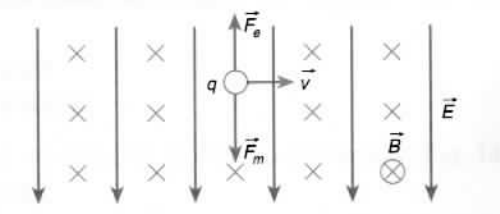
\includegraphics[width=0.6\linewidth]{Figuras/Ch09/fig11.PNG}}
}

\frame{
	\frametitle{Força magnética sobre uma carga elétrica - Exemplo $\#03$}
	\begin{block}{Resolução}
		\begin{enumerate}[(a)]
			\item Pela regra da mão esquerda, a força magnética deveria apontar para cima. Como pela figura vemos que a mesma está para baixo, podemos concluir que a carga é negativa.
			      \vspace{0.2cm}
			\item $|\vec{F_e}| = |\vec{F_m}| \implies |\vec{E}| \cdot q = q \cdot |\vec{v}| \cdot |\vec{B}| \cdot \sen \theta \implies |\vec{E}| =  |\vec{v}| \cdot |\vec{B}| \cdot \sen\ang{90} \implies |\vec{E}| = |\vec{v}| \cdot |\vec{B}| \implies |\vec{v}| = \dfrac{|\vec{E}|}{|\vec{B}|}$
		\end{enumerate}
	\end{block}
}

\frame{
	\frametitle{Força magnética sobre um condutor percorrido por corrente elétrica}
	\begin{block}{Introdução}
		Um condutor percorrido por corrente elétrica de intensidade $i$ e imerso num campo magnético uniforme de indução $\vec{B}$, fica sujeito a uma força magnética $\vec{F_m}$ resultante da ação do campo magnético sobre as partículas eletrizadas que constituem a corrente elétrica.
	\end{block}
}

\frame{
	\frametitle{Força magnética sobre um condutor percorrido por corrente elétrica}
	\begin{block}{Definição}
		Sabendo que $q = i \cdot \Delta t$ e $v = l/\Delta t$, temos as seguintes características da $\vec{F_m}$ sobre um condutor conduzindo corrente:
		\begin{itemize}
			\item \textbf{Direção}: perpendicular ao vetor campo magnético e corrente $i$.
			\item \textbf{Sentido}: obtido através da regra da mão esquerda.
			\item \textbf{Intensidade}:
			      $$\boxed{|\vec{F_m}| = |\vec{B}| \cdot i \cdot l \cdot \sen \theta}$$
		\end{itemize}
	\end{block}
}

\frame{
	\frametitle{Força magnética sobre um condutor percorrido por corrente elétrica}
	\begin{block}{Regra da mão esquerda}
		A regra da mão esquerda, chamada de “regra da mão esquerda de Fleming”, é usada para encontrar o \textbf{sentido da força magnética}.
		\begin{itemize}
			\item O dedo \textbf{polegar} representa o sentido da força magnética ($\vec{F_m}$).
			\item Já o dedo \textbf{indicador} representa o campo magnético ($\vec{B}$).
			\item O dedo \textbf{médio} indica o sentido da corrente ($i$).
		\end{itemize}
	\end{block}
	\centerline{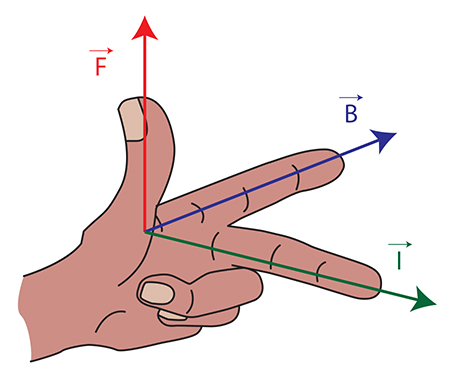
\includegraphics[width=0.45\linewidth]{Figuras/Ch09/fig13.png}}
}

\frame{
	\frametitle{Força magnética sobre um condutor percorrido por corrente elétrica}
	\begin{block}{Observação}
		O ângulo, nesse caso, é formado entre o campo magnético e o comprimento do fio, por isso, ele deve ser \textbf{retilíneo}; caso contrário, teríamos de calcular a força magnética sobre cada trecho do fio que apresentasse um ângulo diferente. Na figura a seguir, temos um fio percorrido por uma corrente elétrica ($i$) em uma região de campo magnético (apontando para fora do plano do papel). Observe o \textbf{sentido da força magnética em cada parte do fio}.
	\end{block}
	\centering
	\setmyunit{0.8cm}
	
	\begin{tikzpicture}
		\pgfmathsetmacro{\len}{0.2}
		\pgfmathsetmacro{\hlen}{\len/2}
		
		\foreach \i in {-2.5,-1.5,...,2.5} {
			\foreach \j in {-2,-1,...,1} {
				\draw[blue] (\i,\j) circle (1ex);
				\fill[blue] (\i,\j) circle (0.5ex);
			}
		}
	
		\draw[blue] (3,0.5) node[] {$ \vec{B} $};
	
		\draw[thick] (-3,-1.5) -- (2,-1.5) -- (2,1.5);
		\draw[-Latex] (-1,-1.5) -- (-1,-2.5) node[left] {$ \vec{F} $};
		\draw[-Latex] (2,-0.5) -- (3,-0.5) node[above] {$ \vec{F} $};
		
		\draw[-Stealth,red] (-2.9,-1.3) -- +(1,0) node[above] {$ i $};
		\draw[-Stealth,red] (1.8,-1.4) -- +(0,1) node[left] {$ i $};
	\end{tikzpicture}

%	\centerline{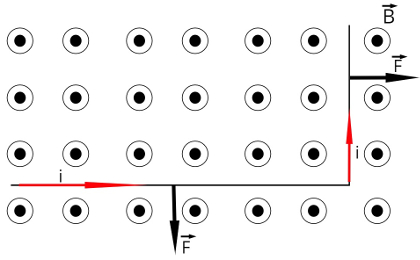
\includegraphics[width=0.5\linewidth]{Figuras/Ch09/fig12.jpg}}
}

\frame{
	\frametitle{Força magnética sobre um condutor percorrido por corrente elétrica}
	\begin{block}{Exemplo $\#01$}
		Uma barra fina de cobre, de comprimento $L = \SI{0.5}{\meter}$ e massa $m = \SI{100}{\gram}$, está inicialmente suspensa por dois fios de massa desprezível. A barra está imersa em campo magnético uniforme e de intensidade $|\vec{B}| =\SI{10}{\tesla}$, cuja orientação é perpendicular e entrando no plano da folha. A gravidade no local possui módulo $|\vec{g}| = \SI{10}{\meter\per\second\squared}$. Para anular a tensão nos fios que suportam a barra de cobre, é necessário que uma corrente $i$ seja aplicada no sentido indicado na figura abaixo. Indique o valor da corrente $i$, em ampères.
	\end{block}

	\centering
	\setmyunit{0.5cm}
	\begin{tikzpicture}
	\pgfmathsetmacro{\len}{0.2}
	\pgfmathsetmacro{\hlen}{\len/2}
	
	\foreach \i in {-10,-9,...,10} {
		\foreach \j in {-2,-1,0,1,2} {
			%				\draw[blue] (\i,\j) circle (0.2);
			\draw[blue] (\i,\j) -- ++(\hlen,\hlen) -- ++(-\len,-\len) ++(0,\len) -- ++(\len,-\len);
		}
	}
	
	\draw[blue] (10.5,-1.5) node {$ \vec{B} $};
	\draw[thick] (-8,0) -- +(0,3.5) (8,0) -- +(0,3.5);
	\draw[line width=5pt,copper] (-8,0) -- (8,0);
	\draw[-Stealth,red] (-2,0.5) -- node[above right] {$ i $} (2,0.5);
	\draw[<->] (-8,3.4) -- node[fill=white] {$ L $} (8,3.4);
	\end{tikzpicture}
}

\frame{
	\frametitle{Força magnética sobre um condutor percorrido por corrente elétrica}
	\begin{block}{Exemplo $\#01$ - Resolução}
		A tensão sobre os fios que sustentam a barra é anulada pela força magnética que surge sobre o fio, de mesmo valor e contrária à força peso. Sendo assim, pode-se igualar a força peso da barra com a força magnética.
		
		$$|\vec{F_m}| = |\vec{P}| \implies |\vec{B}| \cdot i \cdot l \cdot \sen \theta = m \cdot |\vec{g}| \implies i = \dfrac{\num{0,1} \cdot 10}{10 \cdot \num{0,5} \cdot 1} = \SI{0.2}{\ampere}$$
	\end{block}
	\vspace{0.2cm}
}

\section*{Exercícios}
\frame{
	\frametitle{Exercícios}
	\begin{block}{}
		01. Um campo magnético uniforme $\vec{B}$, de módulo \SI{1.2}{\milli\tesla}, está orientado verticalmente para cima no interior de uma câmara de laboratório. Um próton com energia cinética de \SI{5.3}{\mega\electronvolt} entra na câmara movendo-se horizontalmente do sul para o norte. Determine a aceleração do próton ao entrar na câmara. Considere que a massa do próton é $m = \SI{1.67e-27}{\kilogram}$, e que $\SI{1}{\electronvolt} = \SI{1.6e-19}{\joule}$.

		\vspace{0.5cm}

		02. Um fio condutor retilíneo tem comprimento $L = \SI{16}{\meter}$ e transporta uma corrente elétrica contínua, igual a $i = \SI{0.5}{\ampere}$, em um local onde existe um campo magnético perpendicular e uniforme, cujo módulo vale $|\vec{B}| = \SI{0.25}{\tesla}$. Determine o módulo da força magnética exercida pelo campo magnético sobre o fio.
	\end{block}
}

\section*{Referências}
\frame{
	\frametitle{Referências e Exercícios Complementares}
	\begin{itemize}
		\item ALEXANDRE, Charles K.; SADIKU, Matthew N. O. Fundamentos de Circuitos Elétricos. 5. ed. Porto Alegre: AMGH, 2013.
	\end{itemize}
	%\centering{\alert{Página 36 - \textbf{1.6.1 até 1.6.5, 1.6.17 até 1.6.19}}} \\
	\centering{\alert{Lista de exercícios 09}}
}
